% \begin{document}
\chapter{Probabilita' Condizionata}

Cosa significa a livello di calcolo conoscere un nuovo evento?

Notazione:
\begin{itemize}
  \item $ \mathbb{P}(A|B) $: probabilita' dell'evento $ A $ condizionata a $ B $
\end{itemize}

Domanda: se so che si e' verificato $ B $, come cambia $ \mathbb{P}(A) $?

\nt{
  $ \mathbb{P}(A|B) = \mathbb{P}(\cdot | B), B \subseteq \Omega $, quindi essendo sempre una probabilita' ha sempre tutte le proprieta' di una qualunque probabilita'. La probabilita' e' sempre relativa ad $ A $, la $ B $ cambia solo come agisce $ \mathbb{P} $
}

\ex{Probabilita' uniforme}{
  Lancio del dado: $ \Omega = \{1,2,3,4,5,6\} $, $ \mathbb{P} $ prop. uniforme

  $ \mathbb{P}(\{\omega\}) = \frac{1}{|\Omega|}, \forall \omega \in \Omega $, ovvero:
  \[
    \mathbb{P}(A) = \frac{\text{casi favorevoli in }A}{\text{casi possibili}}
  \]
  $ A = \text{"esce un numero maggiore di 3"} = \{3,4,5,6\} $ e $ B = \{\text{"esce un numero pari"}\} = \{2,4,6\} $, domanda $ \mathbb{P}(A|B) $?

  $ P(A) = \frac{4}{6} $ come abbiamo gia visto.

  Ora facciamo che sappiamo che $ B $ si sia avverato. ATTENZIONE! cio' non vuol dire che cambia lo spazio campionario perche' l'esperimento e' lo stesso, ma cambiano i \textit{veri} casi favorevoli e i \textit{veri} casi possibili:
  \[
    P(A|B) = \frac{\text{"veri casi favorevoli di A"}}{\text{veri casi possibili}} = \frac{|A \cap B|}{|B|} = \frac{2}{3}
  \]

  Dado a 4 facce truccato: 

  \[
    \mathbb{P}(A|B) = \frac{\text{"probabilita' dei veri casi favorevoli di A"}}{\text{probabilita' dei veri casi possibili}} = \frac{}{}
  \]
}

\dfn{Probabilita' Condizionata}{
  Prendo due eventi $ A, B $, uno spazio di probabilita' $ \left( \Omega, \mathbb{P} \right) $ con 
  \[
    \mathbb{P}(B) > 0
  \]
  Definisco \textit{probabilita' condizionata a B di A} la funzione:
  \[
    \mathbb{P}(A|B) = \frac{\mathbb{P}(A \cap B)}{\mathbb{P}(B)}
  \]
}

\nt{
  Se $ \mathbb{P} $ e' la probabilita' uniforme allora:
  \[
    \mathbb{P}(A|B) = \frac{\mathbb{P}(A \cap B)}{\mathbb{P}(B)} = \frac{\frac{|A \cap B|}{|\Omega|}}{\frac{|B|}{|\Omega|}} = \frac{|A \cap B|}{|B|}
  \]
}

\nt{
  B e' fissato nella definizione di propbabilita' condizionata, ovvero:
  \[
    \mathbb{P}(A|B) \neq \mathbb{P}(B|A)
  \]
  Quindi il ruolo di $ A $ e $ B $ e' completamente diverso
}

\nt{
  Se $ B = \Omega $, allora $ \mathbb{P}(A|B) = \mathbb{P}(A) $ dato che la conoscenza del fatto che si e' avverato $ \Omega $ e' ovvio e non ci cambia.

  Se $ A = \Omega $, allora $ \mathbb{P}(\Omega | B) = 1 $ (per proprieta', dato che e' sempre una probabilita')
}

Verifichiamo gli assiomi (fissiamo $ B \subseteq \Omega $ con $ \mathbb{P}(B) > 0 $):

\begin{enumerate}
  \item $ \mathbb{P}(A|B) \in [0,1], \forall A \subseteq \Omega $
  \item $ \mathbb{P}(\Omega|B) = 1 $
  \item $ \sigma-\text{addittivita'} $: $ (A_i)_{i \in \mathbb{N}} $ disgiunti:
    \[
      \mathbb{P}(\bigcup_{i=1}^{\infty} A_i|B) = \sum_{i=1}^{\infty} \mathbb{P}(A_i|B)
    \]
\end{enumerate}

\nt{
  La probabilita' condizionata in genere e' nota e si usa per calcolare la probabilita' dell'intersezione:
  \[
    \mathbb{P}(A \cap B) = \mathbb{P}(A|B) \cdot \mathbb{P}(B)
  \]
  Questa formula e' detta regola della catena. Vale in generalecon $ n $ eventi
}

\mprop{}{
  $ (A_i)_{i = 1,...,n}, \mathbb{P}(A_1 \cap ... \cap A_{n-1}) > 0 $, allora:
  \[
    \mathbb{P}(A_1 \cap ... \cap A_n) = \mathbb{P}(A_1)\mathbb{P}(A_2|A_1)\mathbb{P}(A_3|A_1 \cap A_2) ... \mathbb{P}(A_n| A_1 \cap ... A_{n-1})
  \]
  La condizione funziona grazie alla monotonia, dato che $ 0 < \mathbb{P}(A_1 \cap ... \cap A_{n-1}) \leq \mathbb{P}(A_1 \cap ... \cap A_j), 1 \leq j \leq n-1 $
}

\section{Eventi indipendenti}
Si osservi la seguente definizione
\dfn{Eventi indipendenti}{
  Due eventi $ A, B $ si dicono indipendenti se:
  \begin{equation}
    \mathbb{P}(A \cap B) = \mathbb{P}(A) \cdot \mathbb{P}(B)
  \end{equation}
  

  E viene denatato $A \dperp B$
}

Generalizzando: 
\dfn{Eventi indipendenti generale}{
  Sia dati $n$ eventi $A_1, A_2, ..., A_n$, essi si dicono indipendenti se:
  \[
    \mathbb{P}(A_1 \cap ... \cap A_n) = \mathbb{P}(A_1) \cdot ... \cdot \mathbb{P}(A_n)
  \]
  
}

L'indipendenza tra due eventi e' una relazione simmetrica, ovvero:
\[
  A \dperp B \iff B \dperp A
\]

In particolare si noti il seguente teorema:
\thm{Teorema della simmetria tra eventi indipendenti}{ \label{thm:simmetria_indipendenza}
  Sia $\mathbb{P}(B)>0$ allora:
  \[
    A \dperp B \iff \mathbb{P}(A|B) = \mathbb{P}(A)
  \]
  Dall'altro lato, sia $\mathbb{P}(A)>0$ allora:
  \[
    A \dperp B \iff \mathbb{P}(B|A) = \mathbb{P}(B)
  \]
}

\pf{Dimostrazione}{
  Verrà fornita solo la dimostrazione del primo punto, la seconda parte è analoga.

  Assumo $\mathbb{P}(B)>0$, si ha:
  \begin{itemize}
    \item $ A \dperp B \implies \mathbb{P}(A|B) = \mathbb{P}(A) $:
      \[
        \mathbb{P}(A|B) = \frac{\mathbb{P}(A \cap B)}{\mathbb{P}(B)} = \frac{\mathbb{P}(A) \cdot \mathbb{P}(B)}{\mathbb{P}(B)} = \mathbb{P}(A)
      \]
    \item $ \mathbb{P}(A|B) = \mathbb{P}(A) \implies A \dperp B $:
      \[
        \mathbb{P}(A \cap B) = \mathbb{P}(A|B) \cdot \mathbb{P}(B) = \mathbb{P}(A) \cdot \mathbb{P}(B)
      \]
  \end{itemize}
}

\nt{
  Si noti che se $\mathbb{P}(A)>0$ e $\mathbb{P}(B)>0$ allora, le tre uguaglianze seguenti sono equivalenti:
  \[
    \mathbb{P}(A\cap B) = \mathbb{P}(A) \cdot \mathbb{P}(B) \iff \mathbb{P}(A|B) = \mathbb{P}(A) \iff \mathbb{P}(B|A) = \mathbb{P}(B)
  \]
}

Adesso fornirò un altro teorema piuttosto importante:
\mprop{Sull'indipendenza di eventi complomentari}{
  Siano $A, B$ due eventi indipendenti, allora:
  \[
    A \dperp B \iff A^c  \dperp B,\, A \dperp B^c,\, A^c \dperp B^c
  \]
}
\pf{Dimostrazione}{
  Dimostro solo la prima parte, le altre sono analoghe.

  Assumo $A, B$ due eventi indipendenti, debbo dimostrare la seguente uguaglianza:
  \[
    \mathbb{P}(A^c \cap B) = \mathbb{P}(A^c) \cdot \mathbb{P}(B)
  \]

  Dato che 
  \[
    B = \Omega \cap B = (A \cup A^c) \cap B = (A \cap B) \cup (A^c \cap B)
  \]

  E dato che $ (A \cap B) $e$ (A^c \cap B)$ sono disgiunti, per \ref{item:finite_additivity} (\textit{additività finita}) si ha:
  \[
    \mathbb{P}(B) = \mathbb{P}(A \cap B) + \mathbb{P}(A^c \cap B)
  \]

  E dato che $ A \dperp B $ si ha:
  \[
    \mathbb{P}(B) = \mathbb{P}(A \cap B) + \mathbb{P}(A^c \cap B) = \mathbb{P}(A \cap B) = \mathbb{P}(A) \cdot \mathbb{P}(B) + \mathbb{P}(A^c \cap B)
  \]
  Quindi:
  \[
    \mathbb{P}(A^c \cap B) = \mathbb{P}(B) - \mathbb{P}(A \cap B) = \mathbb{P}(B) - \mathbb{P}(A) \cdot \mathbb{P}(B) = \mathbb{P}(B) \cdot (1 - \mathbb{P}(A)) = \mathbb{P}(A^c) \cdot \mathbb{P}(B)
  \]
}

\ex{Calcolo di eventi indipendenti con probabilita condizionata}{

\textbf{TESTO:}

    Si lancia un dado a 6 facce

    \( A = \) "Esce un numero \( > 4 \)" \\
    \( B = \) "Esce un numero pari"

    Determinare \( P(A) \) e \( P(A|B) \)

\textbf{DETTAGLIO SVOLGIMENTO:}

    \begin{align*}
        \Omega &= \{1, 2, 3, 4, 5, 6\} \\
        A &= \{ 5, 6\} \\
        B &= \{2, 4, 6\} \\
        P(A) &= \frac{3}{6} = \frac{1}{3} \\
        P(A|B) &= \frac{P(A \cap B)}{P(B)} = \frac{\frac{1}{6}}{\frac{3}{6}} = \frac{1}{3}
    \end{align*}

    Dato che \( P(A) = P(A|B) \), per il teorema \ref{thm:simmetria_indipendenza} si ha che \( A \dperp B \)
}

Ecco un altro eserzio:
\ex{}{
  \textbf{TESTO}

Lanciamo una moneta e un dado a 4 facce.

Determinare uno spazio di prob. che descriva l'esperimento aleatorio

\textbf{SOLUZIONE}

\Omega = \left\{ (T,1), (T,2), (T,3), (T,4), (C,1), (C,2), (C,3), (C,4) \right\}

P(T,1) = \frac{1}{8} = P(C,4) = \frac{1}{8}

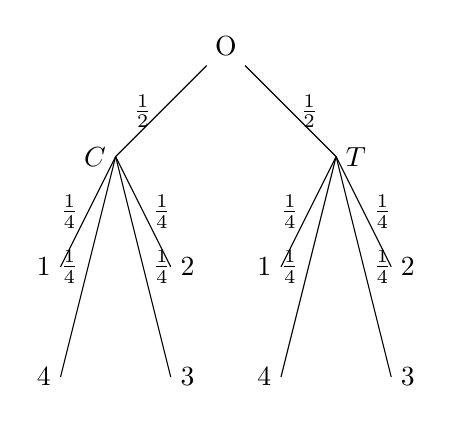
\begin{tikzpicture}[scale=0.7]
    \node (root) at (0,0) {O};
    \draw (root) -- (-2,-2) node[left] {$C$} node[midway,left] {$\frac{1}{2}$};
    \draw (root) -- (2,-2) node[right] {$T$} node[midway,right] {$\frac{1}{2}$};
    
    \draw (-2,-2) -- (-3,-4) node[left] {$1$} node[midway,left] {$\frac{1}{4}$};
    \draw (-2,-2) -- (-1,-4) node[right] {$2$} node[midway,right] {$\frac{1}{4}$};
    \draw (-2,-2) -- (-1,-6) node[right] {$3$} node[midway,right] {$\frac{1}{4}$};
    \draw (-2,-2) -- (-3,-6) node[left] {$4$} node[midway,left] {$\frac{1}{4}$};
    
    \draw (2,-2) -- (1,-4) node[left] {$1$} node[midway,left] {$\frac{1}{4}$};
    \draw (2,-2) -- (3,-4) node[right] {$2$} node[midway,right] {$\frac{1}{4}$};
    \draw (2,-2) -- (3,-6) node[right] {$3$} node[midway,right] {$\frac{1}{4}$};
    \draw (2,-2) -- (1,-6) node[left] {$4$} node[midway,left] {$\frac{1}{4}$};
\end{tikzpicture}

  \[
  \begin{aligned}
  & T = \text{"esito del lancio moneta e testa"} \\
  & C = \text{"esito del lancio moneta è croce"} \\
  & D_i = \text{"è uscito il numero } i \text{"} \\
  & P(C) = \frac{1}{2}, \quad P(T) = \frac{1}{2} \\
  & P(D_i | C) = \frac{1}{4} \\
  & P(D_i | T) = \frac{1}{4} \\
  & A = \text{"è uscito testa e il numero } i \text{"} \\
  & P(A) = P(T) \cdot P(D_i | T) = \frac{1}{2} \cdot \frac{1}{4} = \frac{1}{8} \\
  & \text{Analogamente per } C \cap D_i
  \end{aligned}
  \]
}



% \end{document}
